\section{Technischer Aufbau}
Flash-Speicher basiert auf sogenannten Floating Gate-Transistoren (FGFET). Die Basis für diese sind die sogenannten Metal-Oxid-Halbleiter-Feldeffekttransistoren, kurz MOSFET. In diesem Kapitel wird der physikalische Aufbau zuerst des MOSFETs und anschließend des Floating Gate-Transistors eingegangen. Die Funktionsweise wird im folgenden Kapitel \ref{sec:funktion} beschrieben.

\subsection{Metal-Oxid-Halbleiter-Feldeffekttransistor}
\begin{figure}[h]
    \centering
    \caption{MOSFET als Bauteil}
    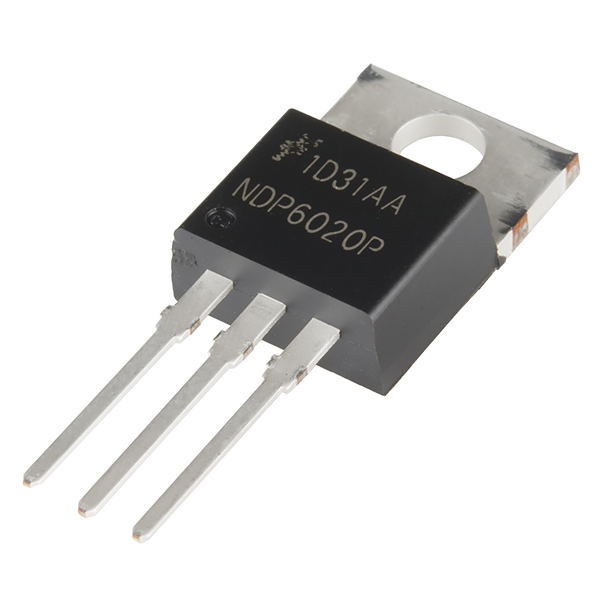
\includegraphics[width=5cm]{sections/img/mosfet_bauteil}
    \label{fig:mosfet.bauteil}
    \\ Quelle: \cite{mosfetshop}
\end{figure}

Ein MOSFET besteht aus einer Art Grundplatte, welche aus einer \gls{pdotiert}en Siliziumeinkristal als Substrat besteht. In dieses Substrat befinden sich zwei stark \gls{ndotiert}e Inseln in denen sich die \emph{Source}-\footnote{dt.: Quelle} und \emph{Drain}\footnote{dt.: Abfluss}-Elektroden befinden. Der Bereich zwischen den beiden Elektroden ist das \gls{pdotiert}e Substrat. Dadurch ist ein Stromfluss zwischen den beiden Elektroden grundsätzlich nicht möglich.

\begin{figure}[h]
    \centering
    \caption{Aufbau eines MOSFETs}
    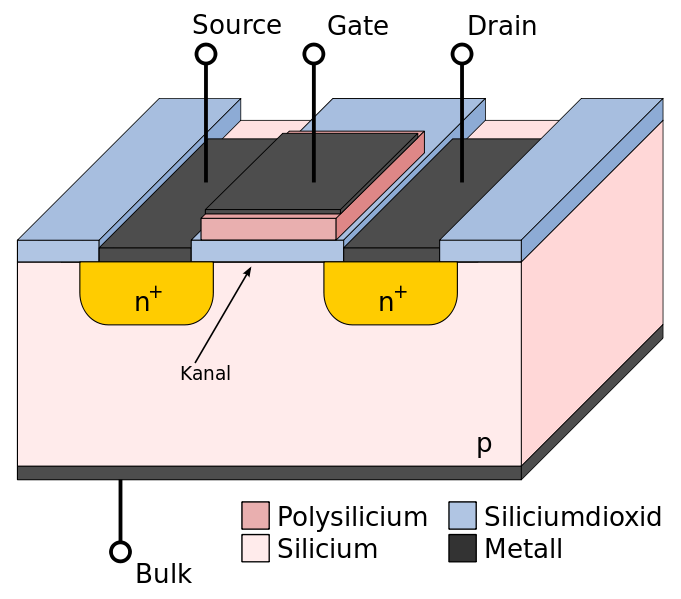
\includegraphics[width=5cm]{sections/img/mosfet_aufbau}
    \label{fig:mosfet.aufbau}
    \\ Quelle: \cite{mosfetwiki}
\end{figure}

Über der Fläche befindet sich eine dünne, isolierende Schicht -- meistens aus Siliziumdioxid. auf dieser Isolierschicht befindet sich dann ein Gate-Material aus \gls{dotiert}em Polysilizium.

\subsection{Floating Gate-Feldeffekttransistor}\label{sec:fgfet}
Die Speicherzellen in Flash-Speicher bestehen aus Floating Gate-Feldeffekttransistoren, kurz FGFET. Diese sind eine Art Weiterentwicklung der MOSFET.

Der Aufbau des FGFETs ist dem des MOSFET sehr ähnlich, allerdings befindet sich zwischen dem Substrat und der Gate-Elektrode noch eine weitere Schicht, das so genannte \emph{Floating Gate}.

\begin{figure}[h]
    \centering
    \caption{Aufbau eines Floating Gate-Transistors}
    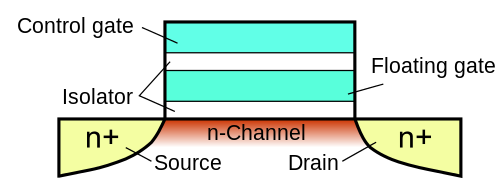
\includegraphics[width=5cm]{sections/img/fgfet_aufbau}
    \label{fig:fgfet.aufbau}
    \\ Quelle: \cite{fgfetwiki}
\end{figure}

Der Name \emph{Floating Gate} stammt daher, dass es rundherum komplett eletrkisch isoliert ist. Es schwebt elektrisch gesehen zwischen der oberen Isolationsschicht des Substrates und der Gate-Elektrode.